\documentclass{article}
\usepackage[T1]{fontenc}
\usepackage[utf8]{inputenc}
\usepackage[margin=1in]{geometry}
\usepackage{fancyhdr} 
\usepackage{listings}
\usepackage[ruled,vlined]{algorithm2e}
\usepackage{amsthm}
\usepackage{amsfonts}
\usepackage{amssymb}
\usepackage{graphicx}
\usepackage[dvipsnames]{xcolor}
\usepackage{xy}
% \usepackage{url} % Commented out because hyperref provides similar functionality
\usepackage{parskip}
\usepackage{comment}
\usepackage{setspace}
\usepackage{enumerate}
\usepackage{multirow}
\usepackage{hyperref}
\usepackage{caption}
\usepackage{subcaption}
\usepackage{booktabs}
\usepackage{wrapfig}
\usepackage{times}

\captionsetup[figure]{font={small,it}}

\usepackage[backend=biber,style=numeric,sortcites,maxbibnames=99]{biblatex}
\addbibresource{references.bib}

\newcommand{\HRule}{\rule{\linewidth}{0.5mm}}
\newcommand{\Hrule}{\rule{\linewidth}{0.3mm}}
\newcommand{\classnum}{CS-GY 6313 B}

\makeatletter% since there's an at-sign (@) in the command name
\renewcommand{\@maketitle}{%
  \parindent=0pt% don't indent paragraphs in the title block
  \centering
  {\Large \bfseries\textsc{\@title}}
  \HRule\par%
  \textit{\@author \hfill \classnum}
  \par
}
\makeatother% resets the meaning of the at-sign (@)

\title{Assignment \#2: Misleading Visualization}

\author{Ivan Aristy}
% \classnum

\begin{document}
  \maketitle % prints the title block
  \thispagestyle{empty}
  % \vspace{-15pt}

References to papers and books look like this \cite{munzner2014visualization}. 

References to sections look like this: \autoref{sec:sec1}

References to figures look like this: \autoref{fig:fig1}

\begin{figure}[ht] % Change the position of your figure https://www.overleaf.com/learn/latex/Positioning_images_and_tables
    \centering
    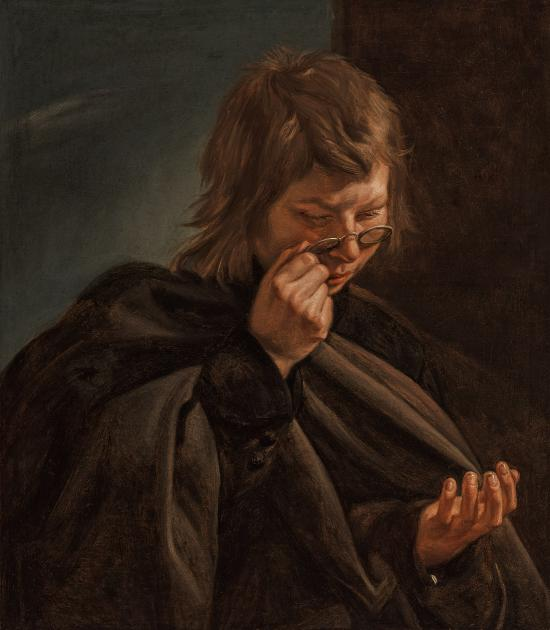
\includegraphics[width=0.75\textwidth]{figs/sight.jpg}
    \caption{
        Figure captions look like this. You can change the size of the figure using the \texttt{width} parameter in the \texttt{\textbackslash includegraphics} command. You can change the position of the figure using the position arguments in the \texttt{\textbackslash begin\{figure\}} environment command.
        URLs look like this: \url{https://www.mfa.org/exhibition/michaelina-wautier-and-the-five-senses}
    }
    \label{fig:fig1}
\end{figure}

\section{Visualizations}
\label{sec:sec1}

The following are the two Visualizations that I have created for this Assignment:

% \begin{figure}[ht] 
%   \centering
%   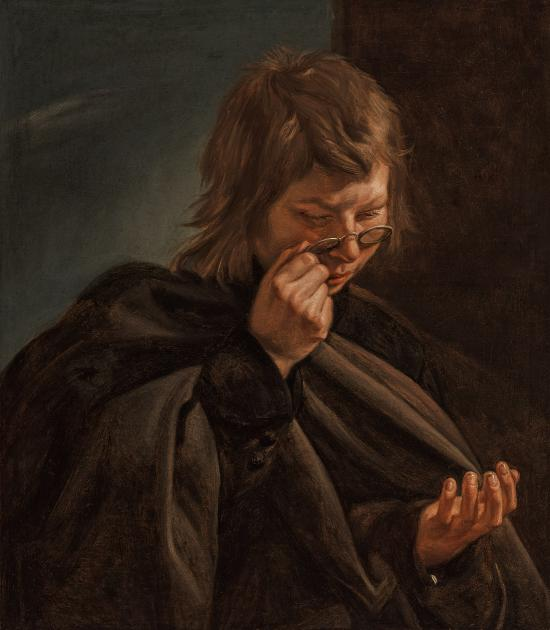
\includegraphics[width=0.75\textwidth]{figs/sight.jpg}
%   \caption{
%       Visualization \#1
%   }
%   \label{fig:Visualization1}
% \end{figure}

% \begin{figure}[ht] 
%   \centering
%   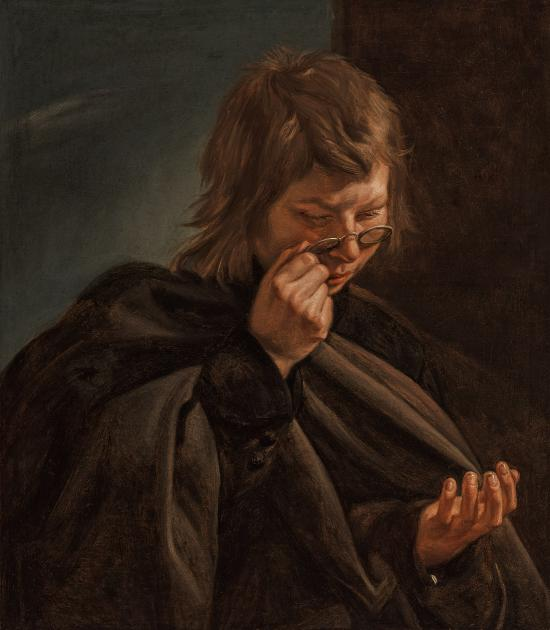
\includegraphics[width=0.75\textwidth]{figs/sight.jpg}
%   \caption{
%       Visualization \#2
%   }
%   \label{fig:Visualization2}
% \end{figure}

\section{}
\label{sec:sec2}

\subsection{Misleading Visualization}
\label{subsec:misleading}

\subsubsection{Topic Ideation}

For the Misleading visualization I had a few ideas:

\begin{itemize}
  \item Immigration and Crime correlations: 
  Showing an extrapolated correlation between immigration and crime rates 
  could be made misleading by selecting data points that support a biased narrative.
  For example, not filtering by region, and actively sampling from regions with high crime rates.

  \item Ethnically Biased Drug Usage: 
  Using the "US Drug overdose death rates, by drug type, sex, age, race, and Hispanic origin" 
  \cite{drugOverdoseDeathRates} dataset, we could use missleading bar charts to exaggerate the 
  correlation between hispanic heritage and drug consumption. Additionally, by 
  filtering out specific drugs we could make it especially misleading.

  \item Presidential Employment Claims:
  As much as I do not like Trump, which you'll see in the extra credit,
  the high employment rates during his presidency are largely do to the Covid-19 pandemic.
  We could use a line chart to show the employment rates over time, in contrast/comparison to Biden, 
  and by not clarifying the context of the data, we could make it seem like Trump 
  was solely responsible for the high employment rates.

  \item Immigration Crisis and Democratic Party Correlation:
  We could use a line graph to show the number of border crossings over time, and, by comparing
  Biden's and Trump's presidency, we could make it seem like the Democratic party is solely 
  responsible for the immigration crisis. This could be further exaggerated by not showing the
  Covid-19 pandemic context, and/or picking legal border crossings to be also part of the data using
  the "Border Crossing Entry Data" \cite{borderCrossingEntryData} dataset. 
  
  \item The Cost of Living vs Inflation: 
  The relation between the American people's expenditures, home prices, income, and inflation rates
  are great for generating accurate and misleading content alike. For example, one could
  greatly overvalue the spending power of the American people by not accounting for inflation rates.
  Also, by sampling subsets of the population, we could make homes seem less or more affordable than they are.
\end{itemize}

\subsubsection{Topic Selection and Question}

For the Misleading Visualization I have decided to go with the "The Cost of Living vs Inflation" topic.

The reason why is because cost of living and economic statistics lend themselves to 
both areas of the spectrum of honesty. We can sample and transform numbers 
in multiple ways, incorrecly scale items, and/or dramatize the effects of 
certain politcal movements and policies to create missleading narratives 
on the issues americans care most about.

The question I will be answering is: 
\textit{How has the increase in home prices prevented the average American from buying a home?}

We will first look at the correct visualization of the data, and try to generate a
visualization that creates confusion; downplays, exaggerates, or eliminates inflation,
and/or misrepresents the increase in home prices.

\subsubsection{Iteration}

The first iteration had a focus on correctly plotting home prices vs real income:



\subsubsection{Final Design \& Missleading Qualities}


\newpage
\begin{refcontext}[sorting=nyt]
\printbibliography
\end{refcontext}

\end{document}

